%\documentclass{llncs}
\documentclass{article}

%
% $Id: improve.tex,v 1.1 2006/01/24 05:04:03 vdmtools Exp $
%

%
% PREAMBLE
%

\usepackage{a4wide}
\usepackage{alltt}

% language settings
\usepackage[english]{babel}

% graphics includes
\usepackage{epsfig}
\usepackage{graphicx}
\graphicspath{{figures/}}
\hyphenation{}

%
% BEGIN DOCUMENT
%

\newcommand{\pgldk}
{PGL Consult \\ Miravej 3, S{\o}ften\\
DK-8382 Hinnerup\\ Denmark. \\
\textit{http://www.pglconsult.dk}\\~~email:\,
\texttt{pgl@pglconsult.dk}}
%\email{pgl@pglconsult.dk}}

\newcommand{\chessnl}
{Chess Information Technology BV\\ P.O. Box 5021\\
2000 CA Haarlem\\ The Netherlands. \\
\textit{http://www.chess.nl}\\~~email:\,
\texttt{Marcel.Verhoef@chess.nl}}
%\email{Marcel.Verhoef@chess.nl}}

\newenvironment{vpp}
{\noindent \rule{\columnwidth}{0.5pt} \begin{alltt}}
{\end{alltt} \rule{\columnwidth}{0.5pt}}

\begin{document}

% use empty page style
\pagestyle{plain}

% the title page
\title{Improvement Suggestions for VDMTools \\
\small{($Revision: 1.1 $ -- \today)}}
\author{Peter Gorm Larsen\\ \pgldk \and Marcel Verhoef\\\chessnl}
%\author{Peter Gorm Larsen\,\inst{1} \and Marcel Verhoef\,\inst{2}}
%\institute{\pgldk \and \chessnl}
\date{\mbox{}}
\maketitle

%\newpage

\tableofcontents

\newpage

\section{Introduction}

This memo intends to provide a series of proposals for enhancing VDMTools
in its future innovative development. Because of the main emphasis on
real-time embedded and distributed systems development from the CSK
Corporation, the suggestions made in this memo focus on exactly that:
enhancing VDMTools for development of such systems. The intent is that
CSK Corporation can make use of the body of knowledge from a collection
of VDM tool support experts (mainly placed throughout Europe, both
industrial and academic users of VDMTools) and use them as external
consultants and/or subcontractors. One can imagine this being arranged
under either time-and-material contractual terms or on firm-fixed-price
terms for one or more of the improvements. \\

Historically, VDM and all the other comparable model-oriented formal
specification approaches (e.g. RAISE, Z and B) have primarily been used
for the development of sequential computer based systems. The majority of
formal approaches that have been used for the development of concurrent
computer systems use explicit focus on the channels used for communication
between the processes (e.g. CCS and CSP). A number of the formal approaches
have been extended in different ways to include a notion of time (e.g. Timed
CSP and the VICE VDM++ version). However, virtually none of the existing
formal approaches are able to deal with combination of concurrency, time
and distributed architecture in a way that would be appropriate for the
development of real-time embedded and distributed systems. This memo
includes suggestions for improving the VICE VDM++ technology with
capabilities enabling exactly this combination and we strongly believe
that if these suggestions are incorporated into VDMTools a really powerful
capability enabling better development of realistic embedded systems will
become available. In particular it will become easy for a specifier to
experiment with different distributed architectures at a very early stage
in the design and thus validate important properties in a cost-efficient
fashion. \\

The VICE (VDM++ In a Constrained Environment) project was supported by
the European Union in collaboration with Matra BAe Dynamics and it was 
carried out shortly before Peter Gorm Larsen left IFAD. This project aimed at
improving the VDMTools capabilities in particular in the real-time embedded
area and a lot of progress was made, but it was never properly commercialised
because of Peter Gorm Larsen�s departure from IFAD. The application used for
a case study in this project was a missile guidance system with a single
processor. Thus, in this project there was not any focus on distribution
between different processors. Nowadays there is however significant more
emphasis on the distributed aspects of real-time embedded systems. The
suggestions made in this memo are thus a continuation of the efforts made
in the VICE project. \\

One of the triggers for this memo is the paper \cite{viceeval}
written by Marcel Verhoef of Chess Information Technology (NL) that was
presented at the first Overture workshop\footnote{This paper is available
at \textit{http://www.cs.ru.nl/research/reports/info/ICIS-R05033.html}.},
entitled \textit{``On The Use of VDM++ for Specifying Real-Time Systems''}.
Marcel is a long-time VDM enthusiast; he made the first version of the
type-checker for VDMTools when he was still a student at the Technical
University Delft (NL) doing his MSc thesis project at IFAD in Denmark
back in 1992. Later, he used VDMTools on several large scale industrial
projects and he is also co-author of the recently published VDM++ book
\cite{vdmbook}. Currently he is part of the BODERC research project at
the Embedded Systems Institute (see \textit{http://www.esi.nl}) where
he works on his PhD thesis. His PhD supervisor is professor Frits Vaandrager
at the Radboud University Nijmegen (NL).\\

In \cite{viceeval}, Marcel took the 6.7.27 version of the VICE tool
and used it to model a large distributed industrial real-time embedded
system (a digital control system for a high-volume office printer). The
paper lists many areas where both the tool as well as the language could
be improved to better fit this class of systems -- in his belief many
changes are mandatory in order to be sufficiently productive and successful
in a commercial environment. The discussion at the conference let to a
joint research session with Peter Gorm Larsen held at Aarhus in October
2005. We reviewed the problems identified and discussed the suggested
solutions. This fruitful session actually let to several more insights
that could solve problems that are not even mentioned in the Overture
paper. \\

Currently, we are targeting a scientific paper for FM'06 that describes
these (language) improvements. Basically, they can be categorised as
follows (in random order):

\begin{itemize}
\item Enhancements to the visualisation capabilities of VDMTools;
\item Enhancements to the static and dynamic analysis capabilities of VDMTools;
\item Enhancements to the VDM++ notation and the corresponding tool support;
\item Improvements to the UML coupling.
\end{itemize}

Prior to presenting the different categories this introduction is followed
by listing the tasks that needs to be carried out to in order to demonstrate
the proof of concept of the improve suggestions made in this memo. Afterwards, 
each improvement category will be detailed further below.  

Finally, this memo is completed by a case study, describing a typical
real-time embedded and distributed system. After introducing the case,
we first show how a suitable VDM++ model can be produced with the
existing VICE VDM++ technology. Then we shown how the VDM++ model
could potentially be formulated and validated with the suggested
improvements. At the end of the VDM++ model using the existing VICE technology
it is also illustrated why it is hard with the currently available
capabilities to discover where potential time requirements are violated
and why this is the case.
We believe that it is very likely that any developments
made with VDMTools for embedded systems has a substantial risks for
failure if the suggested improvements are not realised. Hopefully the
new approach will be able to make it easier to validate such requirements
and when violations are discovered faster to correct the model.



\subsection{Proof of Concept of Enhanced VDM++ Real-Time Features}

In order to assess whether the approach advocated in this memo for 
improving the VDMTools technology in the development of embedded real-time 
and distributed systems, this subsection describes the tasks suggested to 
be carried out to form a proof of concept. These tasks must produce:

\begin{enumerate}
\item An update of the VICE dynamic semantics specification reflecting 
      the suggested 
      semantic modifications in the improved real-time system;
\item A demonstration using the car radio-navigation example shown 
      in this memo about the suggested improvements;
\item An updated scanner and parser that can produce the updated 
      abstract syntax to the dynamic semantics specification;
\item An updated version of ShowVICE that will be able to demonstrate 
      the car radio-navigation example and demonstrate the analysis desirable; 
\item A high level product level functionality description that can be used
      to promote the use of VDMTools for the development of embedded
      real-time and distributed systems using the newly suggested approach; and
\item A guidelines document that at a more technical level is able to 
      provide guidelines as to how the new sugegsted approach with advantage
      can be used for the development of embedded real-time and distributed 
      systems. This document will take the existing guidelines document from 
      the VICE project as a starting point.
\end{enumerate}

It is recommended that the first 5 of these delivarables are produced by 
Peter Gorm Larsen and Marcel Verhoef jointly, whereas the last deliverable 
just as well could be made by Professor Araki's group (and in this way 
probably faster be translated into Japanese).

\subsection{Enhanced visualisation capabilities}

While writing \cite{viceeval}, Marcel already produced a simple off-line
support tool called \textit{``ShowVICE''}. This stand-alone tool is able
to display a UML sequence diagram (with time annotations) of the symbolic
execution of the VICE model.  This functionality is currently lacking
in VDMTools but it is essential for gaining insight into the model,
especially when concurrency and real-time issues come into play.
Such functionality should definitely become an integrated part of
VDMTools and should be enhanced further (for example adding a Gantt-chart
view of the active tasks in the model, showing instance variable evolution
over time etcetera). This kind of functionality provides important input
to the user for validating the correct behaviour of embedded systems.
It would also be valuable to have such sequence diagrams even in the
traditional VDM++ interpreter (without time information). Two screenshots
of the current ShowVice tool are provided in Figure~\ref{fig:sv1} and
Figure~\ref{fig:sv2}.

\begin{figure}[!htb]
\begin{centering}
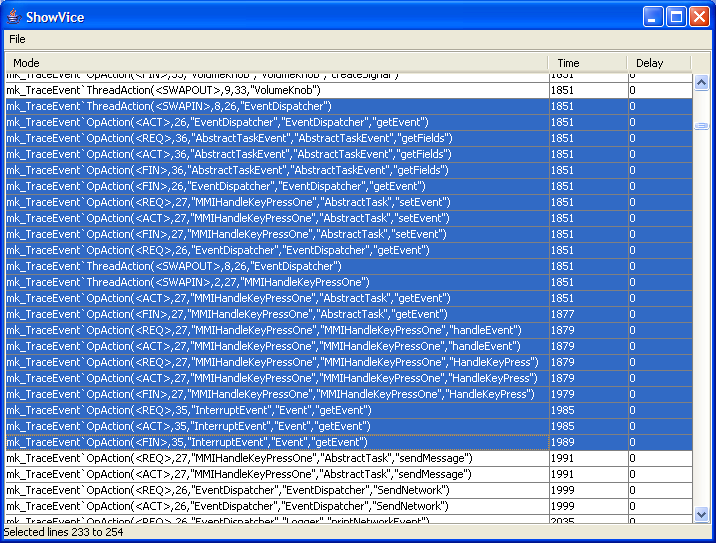
\includegraphics[width=0.80\textwidth]{showvice1.png}
\caption{The main user-interface of ``ShowVICE'', showing a parsed log file.}
\label{fig:sv1}
\end{centering}
\end{figure}

Figure~\ref{fig:sv1} shows an overview of the VICE trace file as it was
read back into the tool from the log file created by VICE after executing
the specification. The user can select the appropriate portion of the log
file that it wants to investigate, which is indicated by the highlighted
part of the list box.

\begin{figure}[!htb]
\begin{centering}
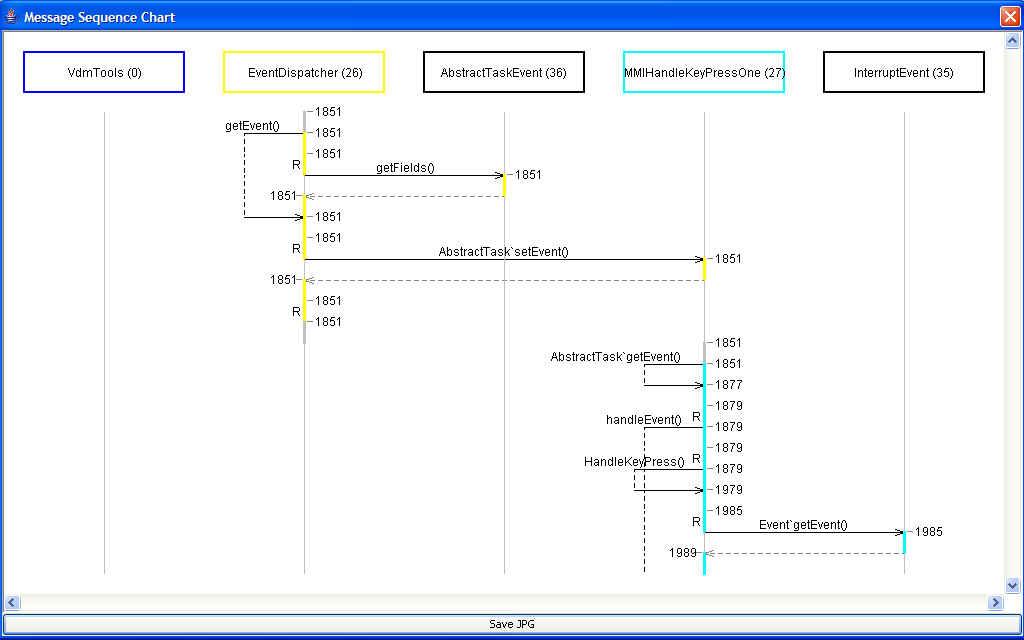
\includegraphics[width=\textwidth]{showvice2.png}
\caption{Detail screen showing a partial time annotated sequence diagram.}
\label{fig:sv2}
\end{centering}
\end{figure}

Figure~\ref{fig:sv2} shows the time annotated sequence diagram of the
selected portion of the trace file. In this particular diagram we see
that a context switch occurs between the \verb+EventDispatcher+ and
the \verb+MMIHandleKeyPressOne+ tasks. Also note that the execution of,
for example, the \verb+Event`getEvent+ operation takes exactly 4 time
units. This graphical feedback is essential to understand the behaviour
of the application. \\

When this kind of functionality is incorporated inside VDMTools, it would
also be extremely valuable to have support for predicates that can be
expressed over these traces. Typically these predicates will be expressed
with universal quantification and relating different events and the times
of their occurrences (inspired by predicates from Real Time Logic 
\cite{Jahanian&86}). It would
be valuable and save time for users if the tool is able to directly
demonstrate the counter-examples that did not satisfy the desired
predicate(s), preferably graphically as shown in Figure~\ref{fig:sv2}.
This is also the main reason why this visualisation functionality should
be integrated into VDMTools and not kept as an off-line inspection tool,
because when a predicate is invalidated, if possible the interpreter should
be stopped immediately such that the cause can be analysed by inspecting
the state of the model graphically as well as using the debugger
command-line. This possibility is obviously not available in the
off-line (post-simulation) based analysis.




\subsection{Increased flexibility for trace file contents}

The trace files produced by the current version of the VICE VDMTools
are not in a format that is appropriate for easy post-analysis because
a proprietary ASCII format is used. The ``ShowVICE'' tool thus has to
parse these trace events before they can be analysed. This
can be solved if the ShowVICE functionality is built into VDMTools as
suggested above. But, the contents of each trace event are still quite
limited, e.g. the arguments for operations invoked are not presented in
the trace file. The reason for that is simple and pragmatic; it would
slow down the execution of the interpreter too much if all information
available inside the interpreter was dumped with each trace event.

Thus, the ideal solution would be to enable the user to select which
information (s)he would like to trace during the simulation and under which
circumstances it should do so. This could, for example, be implemented with
a small scripting language enabling the user to configure the type and the
amount of data to be logged in the trace file and thus be available for
subsequent post-analysis (as a VDM value instead of a proprietary ASCII
format). Some of the timing requirements for an embedded real-time system
may otherwise not be expressible without this feature. An earlier draft of
this note has already led to a significant improvement of VICE. The
\verb+time+ keyword was added to the language, such that simulation
wall clock is accessible from within the specification.




\subsection{Increased support for analysis of deadlocks}

Whenever a deadlock is reached in VDMTools, it can be hard for a
user to determine what the cause of the deadlock is. Thus, the suggestion
is to enable the user to inspect the state of the interpreter in this
situation in a more convenient way. This could for example include:

\begin{itemize}
\item The ability to evaluate / debug the guards (synchronisation
predicates) for the different selected operations that are active in
that context
\item Inspect the value of the history counters for the different
operations in an easy manner
\item The ability to inquire the status of the interpreter scheduler
and all tasks
\end{itemize}




\subsection{Improvement of the VDM++ language}

The VICE notation was recently evaluated by Marcel in his paper
\cite{viceeval} presented at the first Overture workshop explaining the
problems when describing distributed embedded real-time systems with VICE.
The main challenges he identified with the current notation are:

\begin{itemize}
\item The VDM++ notation is by nature synchronous; operation calls are
either blocked on an permission predicate or executed in the context of
the thread of control of the caller (an active object with its own
\verb+thread+ clause in the class definition). This is very cumbersome
when describing embedded systems, which are typically reactive (and 
therefore asynchronous) by nature. Of course, an event loop can be
specified to simulate the asynchronicity, but it would clobber the
specification greatly and lowers the productivity of the user. The
specification is intrinsically bigger than necessary and the validation
of the model is also more complex because of the increased model size.
Users are typically overwhelmed by the amount of run-time data that such
a ``hand-coded'' event loop generates. The language should therefore
allow for \textit{asynchronous} operation calls to overcome this problem. 

\item Similarly, the active object is currently the ``owner'' of the thread
of control. This is ok when all threads are executed on the same processor
(this is the current implementation in VICE) but it really complicates
matters when distributed systems are modelled. Note that when describing
embedded systems, this necessity is paramount, because the environment of
the system can always be viewed as the ``second processor'' that works in
full-parallel to and independent from the embedded system; both have their
own behaviour and (timing) requirements that are only influenced by the
(timed) exchange of stimuli and responses. Therefore, the ownership of the
thread of control should move from the ``active class'' to the (physical
or virtual) processor on which the class instance is deployed. The behaviour
of the system is then determined by the scheduling policy on that processor
and its total capacity (available computing power).  By doing this, it would
be possible to describe deployment of software over a distributed computer
system, also taking into account that one processor might be slower than
another, leading to different response times. This would be a great step
forward; as far as we know this has not been done before and it has a
dramatic practical impact for describing industrial applications, where
most systems nowadays are in fact already multi-processor solutions. 

\item Last but not least, we have some ideas that would also allow
describing the interconnection between the processors (the network) at
a very high-level of abstraction. Inter task communication is now considered
instantaneous in VDM++ (or must be encoded explicitly using duration
statements) which is far from reality. The network deployment view we
envisage gives rise to include communication overhead into the simulation
model at relative little extra cost (for both describing and analysing the
system). In combination with the asynchronous operation calls, all typical
styles of inter processor (and inter task) communication can be described:
synchronous, asynchronous and publish/subscribe, while remaining at a
high-level of abstraction when writing the specification.

\end{itemize}

We believe that these changes can be achieved with limited impact to the
existing syntax and semantics of the language and the tool. We are currently
working on a scientific paper that describes these conceptual changes to the
VDM++ language. This should be seen as a ``proof of concept'' description
that could be used as a guideline to the full-blown implementation in
VDMTools. The first draft of the paper is expected to be ready in
February 2006. A case study illustrating the effect of these suggested
improvements is presented in Sections~\ref{sec:viceorg} and \ref{sec:vicenew}.
However, we do emphasise that this is ``work in progress''. For example,
the specification using the improved language has not been mechanically
verified because tool support is simply lacking.



\subsection{Enhancement of the UML coupling for VDMTools}

The ``Rose link'' was originally made to couple VDMTools with Rational Rose.
Meanwhile, UML has developed substantially and is now an updated standard -
version 2.0. It would be very advantageous for all users of VDMTools that
wish to use VDM++ in conjunction with class diagrams from UML if this new
standard would be adopted. The enhancements could for example include:

\begin{itemize}
\item Rather than being bound to Rational Rose only, the UML link could be
implemented using XMI (the UML model interchange format) such that all UML
tools, that support this exchange standard for UML models, could be used
(including public domain tools). This would remove the current ``vendor
lock-in'' to Rational Rose for VDMTools. This is in particular important
for the real-time and embedded market, where I-Logix Rhapsody seems to
have a much larger market penetration than Rational Rose. 

\item The I-Logix company have produced a system engineering process called
``Harmony'' that seem very appropriate for the development of embedded
real-time systems. This method and the recently released SysML (the Systems
Engineering modelling language, also from the OMG in collaboration with the
International Council of Systems Engineers INCOSE) should be analysed further
for better integration with VDMTools for the early phases of development. 

\item As a minor point, support for packages and hierarchical classes
in UML 2.0 could be taken into account in VDMTools. Similarly, state
transition diagrams from UML could easily be imported into a VDM++ model,
provided that asynchronous operation calls are supported in the language.
\end{itemize}

The round-trip engineering approach advocated by the existing VDMTools
is still very worthwhile in the context of UML\,2.0. The new UML notation
still has no agreed syntax (and semantics) for the specification of
(for example) operations -- which is a natural fit with VDM++, as
described for example in the VDM++ book \cite{vdmbook}. Do note however
that Stephen Mellor is leading an OMG activity currently to define a (new)
language for the creation of executable UML models, something that VDM++
already provides but the majority of UML users is probably not aware of.
To prevent OMG re-inventing the wheel once more (as they did with OCL),
it is suggested that CSK, in collaboration with their academic partners,
makes a case for acceptance of VDM++ as a suitable and already existing
and industry proven solution for the specification of executable UML
models. This should be actively pursued and pushed as soon as possible. \\

OMG also promotes the Model Driven Architecture approach to systems
analysis and design. While the coupling to UML already implements parts
of that strategy, the current VDMTools implementation is not well-suited
for this. It was just not designed with MDA in mind. The Overture open
source initiative (\textit{http://www.overturetool.org}) attempts to
solve part of this problem by providing access to a standardized XML
format for the abstract syntax of VDM specifications. We suggest that
the Overture effort is actively supported from within CSK. Overture is
the ideal platform to get academic researchers involved in the
development of new tools and ideas as proposed in this note. It can
become a breading ground for new ideas and an excellent opportunity
for community building. \\

The above two paragraphs indicate that the current work on UML\,2.0
and MDA is pretty much orthogonal to the improvements to VICE proposed
in this note. These issues are not hampering each other but the
relationship between VDM++, UML and MDA can certainly be strengthened
by implementing the suggested language and tool improvements. In our
opinion, it will also leverage the market potential for VDMTools.



\section{A case study -- using VICE}
\label{sec:viceorg}

The case study presented in this section is used to analyse the performance
of a distributed in-car radio navigation system. The case study was originally
modelled using the Modular Performance Analysis technique, as described in the
paper \textit{``System Architecture Evaluation Using Modular Performance
Analysis -- A Case Study''} by Wandeler et al \cite{orgcase}.
We refer to this paper\footnote{Available at
\textit{http://www.cs.ru.nl/research/reports/info/ICIS-R05005.html}.
Additional information can be found at
\textit{http://people.ee.ethz.ch/$\sim$leiden05/data/pset/p2.pdf}
and at \textit{http://www.mpa.ethz.ch} .} 
for a full description of the case study. 

\begin{figure}[!htb]
\begin{centering}
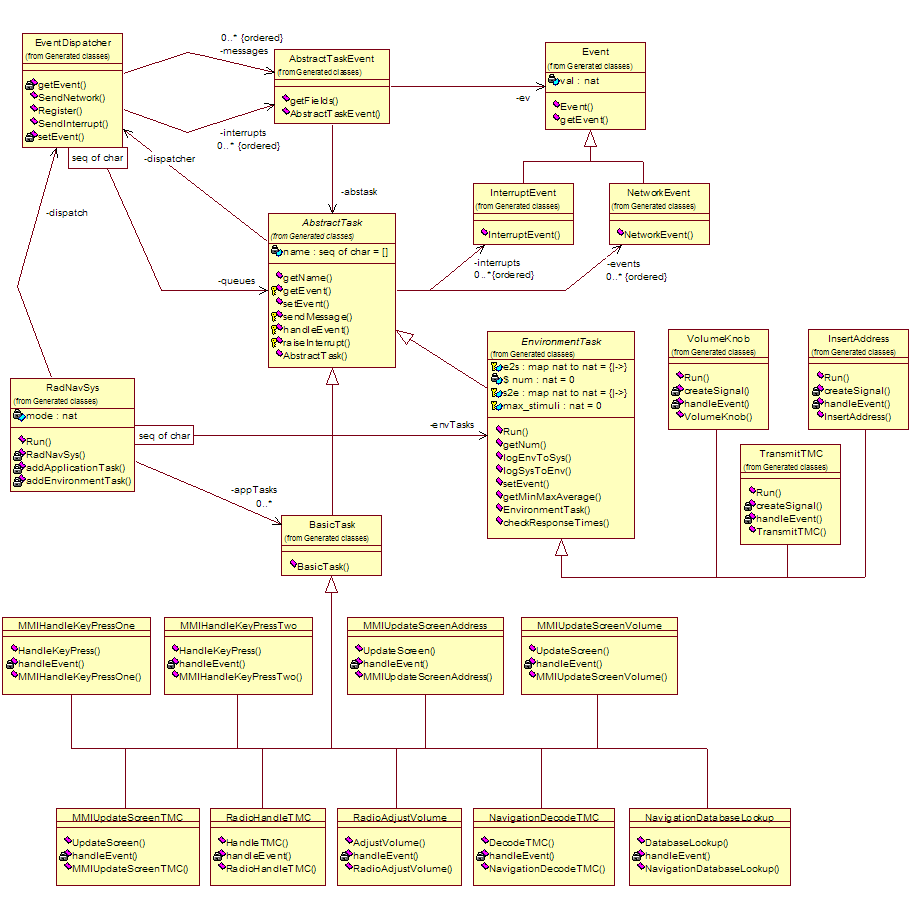
\includegraphics[width=0.8\textwidth]{classold.png}
\caption{UML class diagram of the case study using standard VICE}
\label{fig:uml1}
\end{centering}
\end{figure}

In this note, an attempt was made to describe the same case study using
VDM++, first with the original VICE language and later we will present the
proposed extensions to the language. A UML class diagram of the case study
using the existing VICE technology is shown in Figure~\ref{fig:uml1}.
In Figure~\ref{fig:uml2}, a class diagram of the same case study is shown,
but then using the suggested improvements to the VICE language. It is
immediately clear from those two diagrams that the suggested improvements
significantly reduce the size of the model. But more importantly,
the model using the languages extensions describes the system in
far more detail than the standard VICE specification. The latter can
only describe the single CPU architecture case (and already with some
difficulty because the environment tasks are not really running in
parallel to the embedded system) while the former is able to describe
\textit{all} possible distributed architectures describe in
\cite{orgcase}. Note that our discussions with the CSK team have
already led to changes in the VICE tool. For example, the \verb+time+
keyword was added which allows the user to access the simulation wall
clock of the interpreter directly.

\begin{figure}[!htb]
\begin{centering}
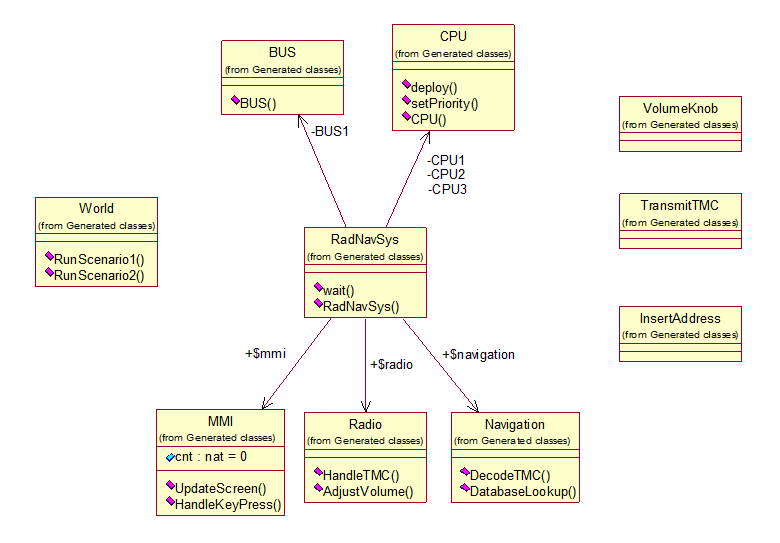
\includegraphics[width=0.6\textwidth]{classnew.png}
\caption{UML class diagram of the case study using the improved VICE notation}
\label{fig:uml2}
\end{centering}
\end{figure}

The in-car radio navigation system is basically a soft real-time system that
executes several concurrent applications at the same time (each consisting
of several tasks), for example for controlling the radio while Traffic Message
Channel data is being processed. Timing requirements are typically specified
per application and the question of interest is whether or not these
requirements are met under all operating conditions, when deployed on
a given architecture. In this note we will consider the situation where all
applications are running on a single CPU, because it is the only configuration
that we can effectively describe using the existing VICE technology. VICE only
supports uni-processor multitasking models, while some architectures considered
in the paper above require a notion of multi-processor multitasking. First, we
will present the model in the existing VICE notation.
In Section~\ref{sec:vicenew} we will present the model
in the improved VICE notation.

\subsection{A mini-framework for reactive systems modelling}

The in-car radio navigation system is a typical real-time embedded system;
it is waiting for stimuli from the environment and processes those events
accordingly. Some stimuli only change the internal system state but most
will cause a response back to the environment. In our case study all
stimuli will cause an external visible response.

Timeliness requirements are often specified in terms of the elapse time
between the stimulus and the response of the system. Such a system is
typically described by an event loop; the system is waiting for stimuli
and when one arrives, it is identified and the appropriate operation is
called and the event loop is immediately resumed. For this to work in
real-time systems, the operation calls shall be asynchronous because
the event loop should never be blocked by the call because it would
potentially delay a high priority event that arrived just after the
event that is currently being processed. Since neither VDM++ nor
VICE supports asynchronous operation calls, we have to mimic this
behaviour by using threads and explicitly describing the event loop.

The Event class is the abstract base class for the events that are managed
by such an event loop. A natural number is used to ``trace'' each individual
event through the system, such that we can specify timing (and temporal)
requirements easily.

\input{Event.vpp.tex}

Two different event types are modelled here: interrupt and network events.
Interrupts are used to trigger the system from the environment, network
events are used to model inter task communication within the system.
As we will see later, interrupts \textit{have priority} over network events.

\input{InterruptEvent.vpp.tex}

\input{NetworkEvent.vpp.tex}

The \verb+AbstractTask+ class provides the basic functionality to handle
events. Two separate input queues are maintained, one for interrupts and
one for network events. There will be a single \verb+EventDispatcher+
instance that will dispatch all system events to the appropriate active
object. The EventDispatcher can raise interrupts or send network events
by calling the public \verb+setEvent+ operation of the applicable
\verb+AbstractTask+ instance. The operations \verb+getEvent+ and 
\verb+handleEvent+ are used to implement the event loop, as we will
see later. Note that \verb+getEvent+ gives priority to interrupts over
network events; calls to the operation will be blocked (because of the
synchronisation predicate) until there is at least one event available.
The \verb+AbstractTask+ can send messages (or raise interrupts) to other
\verb+AbstractTask+s by calling \verb+sendMessage+ or \verb+raiseInterrupt+.
In both cases, the dispatcher will be called to route the message to the
receiving task without blocking the caller.

\input{AbstractTask.vpp.tex}

The \verb+BasicTask+ class implements the event loop. It is an active
object (with its own thread of control) that is constantly processes
incoming events. The task will be blocked when no events are available,
due to the synchronisation predicate specified in the base class.

\input{BasicTask.vpp.tex}

The \verb+EnvironmentTask+ class is used to model tasks in the environment,
outside the scope of the system. EnvironmentTask instances generate the
stimuli for the system and observe the responses coming back. Both stimuli
and responses are administered using the \verb+logEnvToSys+ and 
\verb+logSysToEnv+ operations respectively. The function
\verb+checkResponseTimes+ is used to check the system timeliness
requirements. We will see later how it is used. The operation \verb+getNum+
is used to create unique identifiers, one for each stimulus that is
generated and inserted into the system. Recent discussions with the CSK
team has led to a change in the existing VICE tool already. The \verb+time+
keyword was added to refer to the simulation wall clock of the interpreter.
This feature is used in the \verb+logEnvToSys+ and \verb+logSysToEnv+
operations.

\input{EnvironmentTask.vpp.tex}

\subsection{Modelling the system application tasks}

In this section, the application tasks are listed. There are six tasks
in total. The event loop for each task is simple; the appropriate
synchronous function is called and the next task in the sequence is
signalled by sending a message to it. Note that the time penalty of the
synchronous operation is modelled using the standard VICE duration
statement. First the \verb+MMIHandleKeyPressOne+ class which is used in
scenario~1.

\input{MMIHandleKeyPressOne.vpp.tex}

\noindent Next, the \verb+MMIHandleKeyPressTwo+ class which is used in
scenario~2.

\input{MMIHandleKeyPressTwo.vpp.tex}

\noindent The class \verb+MMIUpdateScreenVolume+ is used in scenario~1
to handle screen updates caused by the volume changes of the radio.

\input{MMIUpdateScreenVolume.vpp.tex}

\noindent The class \verb+MMIUpdateScreenAddress+ is used in scenario~2
to handle screen updates caused by the address lookup actions in the database.

\input{MMIUpdateScreenAddress.vpp.tex}

\noindent The class \verb+MMIUpdateScreenTMC+ is used in both scenarios
to display decoded TMC messages on the screen.

\input{MMIUpdateScreenTMC.vpp.tex}

\noindent The class \verb+RadioAdjustVolume+ is used to adjust the volume
of the radio.

\input{RadioAdjustVolume.vpp.tex}

\noindent The class \verb+RadioHandleTMC+ is used to process incoming TMC
messages over the radio.

\input{RadioHandleTMC.vpp.tex}

\noindent The class \verb+NavigationDatabaseLookup+ is used to search for
an address in the navigation database.

\input{NavigationDatabaseLookup.vpp.tex}

\noindent The class \verb+NavigationDecodeTMC+ is used to decode TMC messages
into a human readable format using the information from the database.

\input{NavigationDecodeTMC.vpp.tex}

\subsection{Modelling the environment tasks}

There are three environment tasks for our case study. One to insert ``key
press'' events (\verb+VolumeKnob+), one to insert ``lookup address'' events
(\verb+InsertAddress+) and one to insert Traffic Message Channel messages
(\verb+TransmitTMC+). The environment inserts these events into the system
by raising an interrupt. Note that all environment tasks exhibit the same
basic structure. The operation \verb+createSignal+ is called periodically
by its own the thread of control to generate the stimulus. Note that we
\textit{have to} use the statement \verb+duration (0)+ explicitly in order
to ensure that the execution of the environment task does not influence
the notion of time of the application tasks in the system model. As a
consequence, we cannot write environment tasks that make use of the
duration statement, for example to insert a second stimulus after
\textit{x} time units, because that would influence the notion of time
of the system model (which is supposed to run in parallel with its ``own''
notion of time). This makes life for the specifier rather difficult in
some cases. The underlying problem is that the uni-processor multitasking
semantics of VICE is \textit{not strong enough} to model both the environment
and the system operating at the same time. We need to move from the
interleaving semantics to true parallel behaviour to describe this properly,
effectively implementing a multi-processor multitasking approach where the
environment task is assigned its own independent processor. \\

Despite this deficiency in VICE, we are still able to express timeliness
properties, as can be seen in the \verb+handleEvent+ operation. Whenever
a response is observed, it is added to the trace information and the
post-condition of the \verb+handleEvent+ operation states that the time
difference between each pair of stimuli and responses shall be less than
some (user-defined) value. Note that there is no completeness requirement
specified here, we can in fact insert more stimuli than we receive back
from the system. This is left out on purpose here; it cannot be checked
on-line because a stimulus might be ``inside'' the system for a very long
time and we are never sure that we waited long enough (this is called the
quiescence property), unless we specify an explicit time-out value for each
expected response. In this specification it is solved by limiting the number
of inserted stimuli and waiting for all responses of all inserted stimuli.
Since the number of stimuli is limited, we know that eventually the system
has enough time to deal with each one. Typically, these kinds of completeness
requirements are processed off-line, after the simulation run is completed;
similarly for temporal properties enforcing some fixed (partial) order in
the stimuli. Another reason for off-line processing might be simulation
efficiency, since the log will increase in size the longer we simulate and
therefore checking the post-condition every time might take up too much
time. When doing post-processing the timeliness, completeness and temporal
requirements only have to be checked once for the trace which makes it
very efficient. \\

Furthermore, we have no explicit control over the start time of the first
period of a periodic task, it is currently dependent on the settings of the
interpreter. This can cause problems because we might know for example that
two otherwise independent environment tasks have the same period but always
run out of phase by some time margin, for example 10 percent of the period.
If the simulator however chooses to activate both periodic tasks right after
one another (remember we use duration zero) that might cause a different
response time behaviour of the system than when the out-of-phase execution
of the environment task was taken into account properly. At the moment,
these kind of problems cannot be handled by the VICE extensions. \\

Another problem is the scheduling of the periodic tasks. Whenever the
periodic task is scheduled, it should become the active task immediately,
pre-empting any other task running, in order to maintain a consistent clock
value. If the periodic task is delayed (or interrupted) by another task that
lets time progress (with some duration greater than zero) then the clock will
become out of sync because we do not know by how much time we were delayed.
If that problem occurs during simulation of the model then the trace files
that are built up here immediately become useless. But more importantly, it
is currently extremely difficult to find out whether or not that problem
actually did occur. So if an invalid trace is detected, is it really an
invalid trace or is it a side-effect of the simulation? \\

\noindent The \verb+VolumeKnob+ class which is used in scenario~1.

\input{VolumeKnob.vpp.tex}

\noindent The \verb+InsertAddress+ class which is used in scenario~2.

\input{InsertAddress.vpp.tex}

\noindent The \verb+TransmitTMC+ class which is used in both scenarios.

\input{TransmitTMC.vpp.tex}

\subsection{Linking everything together -- the event dispatcher}

The EventDispatcher is the most important active object in the specification.
It mediates all the events in the model, both to and from the environment and
to and from the system. Basically, it receives all events, puts them into
temporary queues and greedily dispatches them to the appropriate receivers.
When simulating, the user should ensure that it is the highest priority task
running using pre-emptive scheduling, such that it can process the events
as soon as they become available. The \verb+Logger+ base class is shown in
the appendix. It provides functionality to output the order of the events
that were processed into a file. With the new \verb+time+ keyword it is
now possible to relate this user defined log to the standard log file that
is produced by VICE. Using these two log files in combination can increase
the insight into the model tremendously!

\input{EventDispatcher.vpp.tex}

\subsection{Composing the top-level system model}

The class \verb+RadNavSys+ is the top-level specification for our case-study.
It is used to instantiate and start the model. The system can be analysed
using two different sets of environment tasks exercising the system. The
user can select between the scenarios by supplying the appropriate parameter
to the constructor of the class. For example, the system can be simulated
by calling \verb+new RadNavSys(1).Run()+ on the command-line of VICE.

\input{RadNavSys.vpp.tex}

\subsection{Executing the model}

Before we can execute the model, we have to set up the VICE interpreter.
We use VICE in the pre-emptive scheduling mode, with all options enabled
(dynamic type, invariant, pre- and post-condition checking). The following
task priorities were specified (they are maintained in an external file
called \verb+priority.txt+).

\begin{vpp}
VolumeKnob:10;
InsertAddress:10;
TransmitTMC:9;
EventDispatcher:8;
MMIHandleKeyPressOne:6;
MMIHandleKeyPressTwo:6;
MMIUpdateScreenVolume:5;
MMIUpdateScreenAddress:5;
MMIUpdateScreenTMC:4;
RadioAdjustVolume:3;
RadioHandleTMC:2;
NavigationDecodeTMC:1
\end{vpp}

The environment tasks are given the highest priority, to ensure that they
can indeed inject stimuli whenever their period has expired. Next highest
priority is the \verb+EventDispatcher+ which orchestrates the message
handling between the tasks and the environment. Following are the
application tasks, with priorities as specified in the case study
definition. We can now execute the model using the VICE interpreter.

\begin{vpp}
Initializing specification ...
done
>> priorityfile priority.txt
>> print new RadNavSys(1).Run()
D:/papers/vdmppsem/improve/TransmitTMC.vpp, l. 17, c. 26:
  Run-Time Error 59: The post-condition evaluated to false
>> print e2s, s2e
\{ 1 |-> 2047,3 |-> 3935,4 |-> 4131,6 |-> 5119,8 |-> 6107,10 |-> 7095,
  12 |-> 8083,14 |-> 9071,16 |-> 10059,18 |-> 11047 \}
\{ 1 |-> 25741 \}
\end{vpp}

The VICE interpreter stops in the post-condition of the \verb+TransmitTMC+
operation. We print out the stimuli (e2s) and response (s2e) mappings and
indeed we see that the first stimulus sent actually stayed inside the
system longer than 10000 time units. It is nice that we know that we do
have a problem in our system but can we find the cause of the problem
easily? Actually, that is very hard -- even with the \verb+time+ extension
recently added to VICE. We have to go over the trace files manually, or
use dedicated analysis tools. Even for this simple example the trace file
becomes approximately 300kb, containing several thousands lines of data.
It is clear that powerfull analysis tools are needed to help the user
to better understand the (execution data of the) model.



\input{newcase.tex}

\nocite{*}

\bibliographystyle{splncs}
\bibliography{improve}

\pagebreak

\section*{Appendix -- Auxiliary classes}

\input{Logger.vpp.tex}

\input{AbstractTaskEvent.vpp.tex}

\end{document}
